\chapter{Notas de codificação axial (AC)} %Anexo I (lista as notas AC e seus respectivos conteúdos)
\label{apendice:i_notas_ac}
\section{Notas de codificação axial do Grupo 1 (sem PDTI)}
As páginas a seguir contém as 20 notas do tipo AC criadas durante o desenvolvimento da pesquisa sobre o grupo 1.

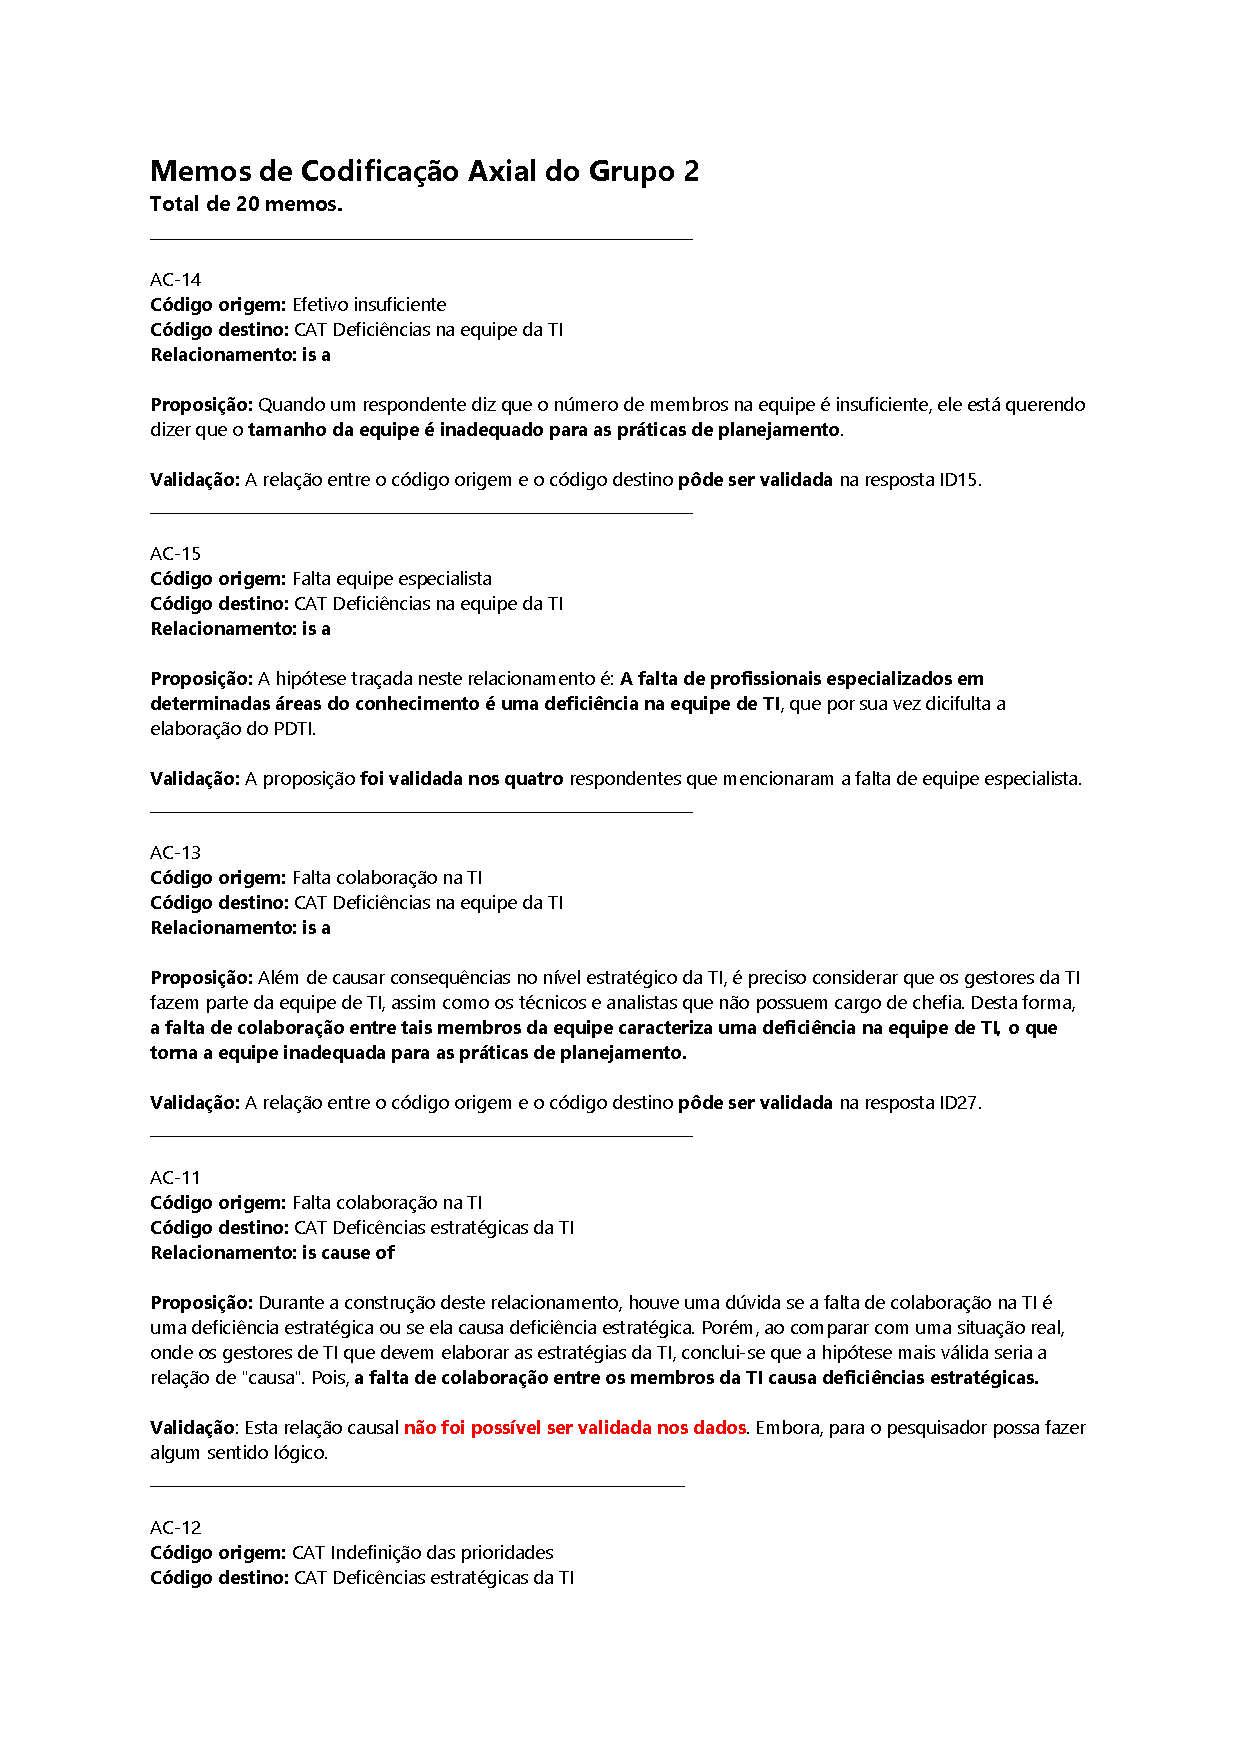
\includepdf[pages=-]{includes/apendiceI_novo_H_AC_g1.pdf}

\section{Notas de codificação axial do Grupo 2 (com PDTI)}
As páginas a seguir contém as 29 notas do tipo AC criadas durante o desenvolvimento da pesquisa sobre o grupo 2.

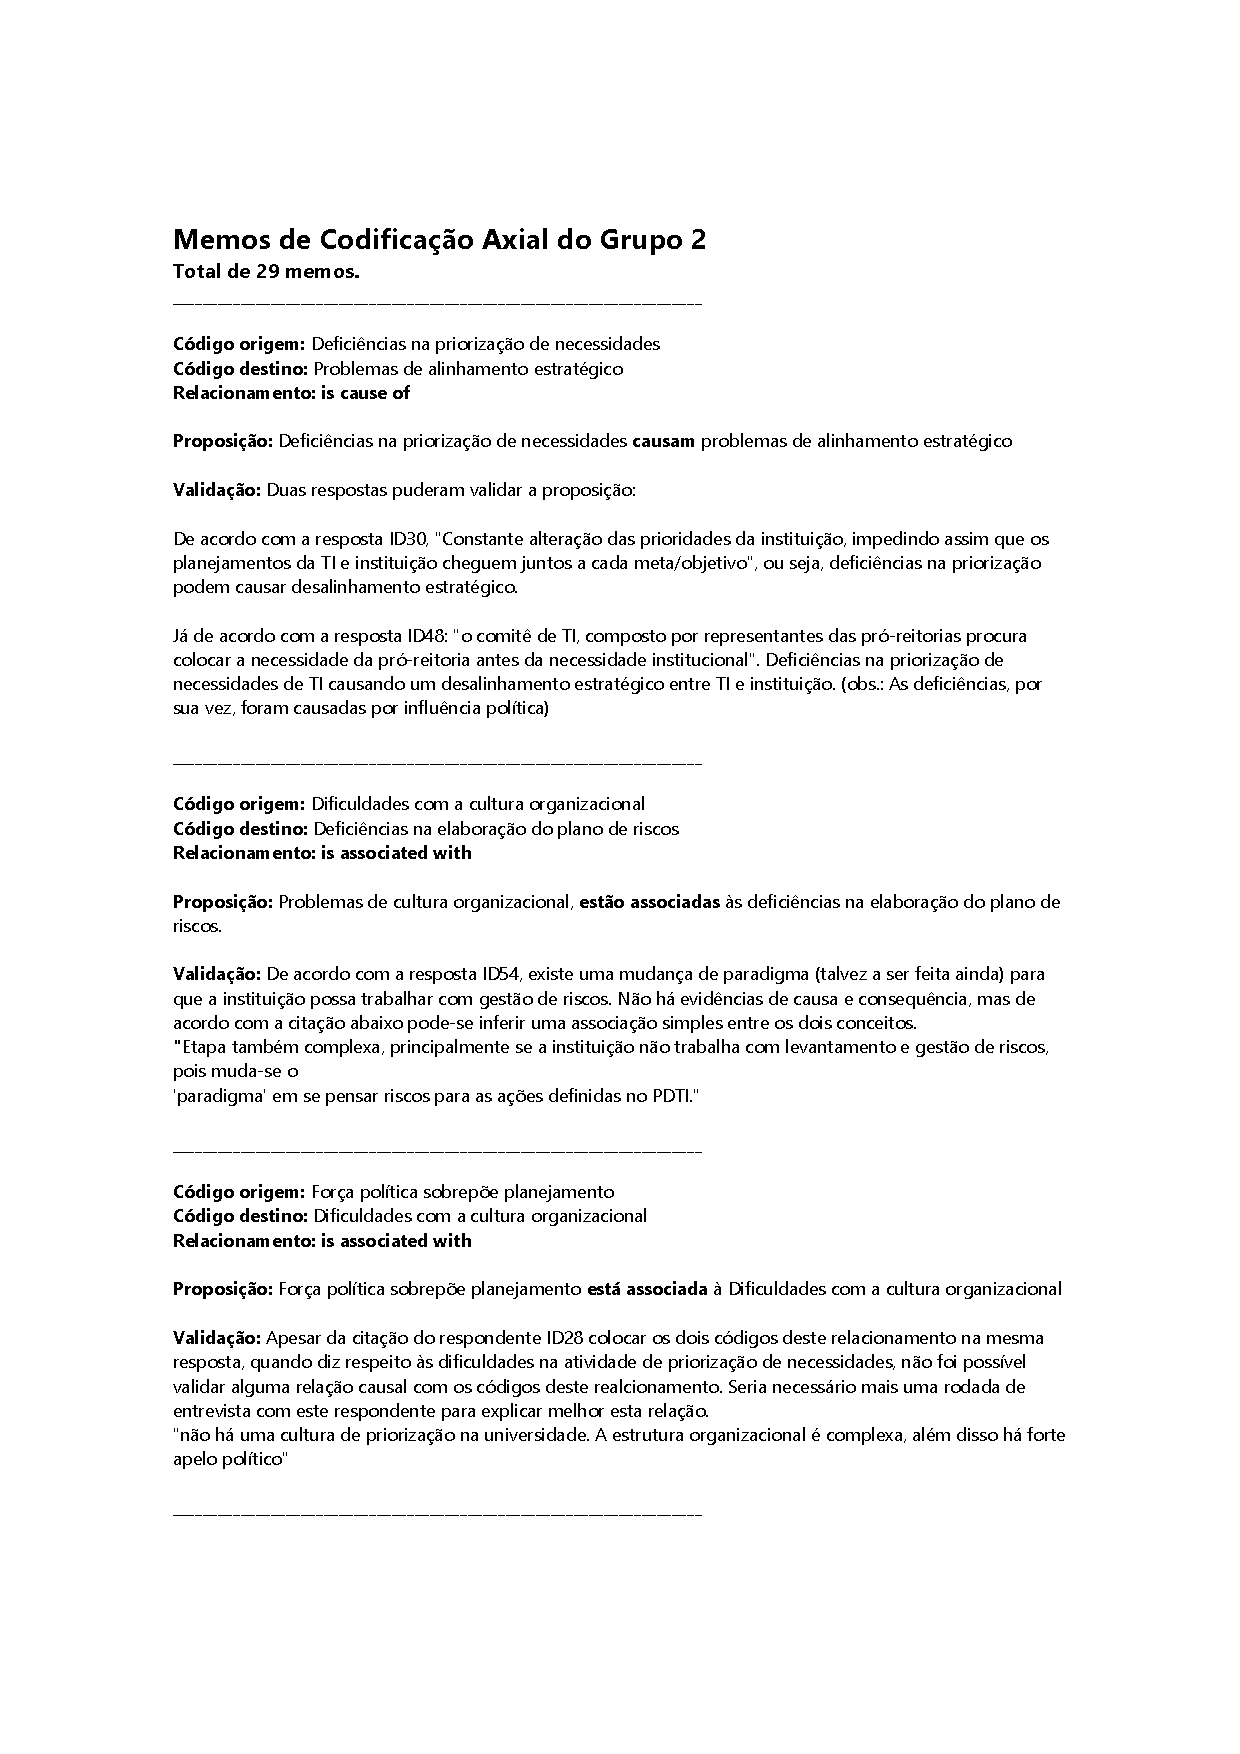
\includepdf[pages=-]{includes/apendiceI_novo_H_AC_g2.pdf}